With the introduced software solutions, the simulation software and the selfish proxy, it is now possible to analyse selfish mining and its impact on the relative gain of the selfish miner.
For the simulation, the scenario described in chapter 45 is adapted.
One of the twenty nodes is eclipsed with the selfish proxy forming a selfish miner.
To obtain a comprehensive overview of the impact of selfish mining the selfish miners conducts various combinations of selfish mining strategies.
Additionally, different distributions of the computation power between the nodes and the selfish miner are applied.

\section{Selfish mining scenarios}

As strategies, the standard selfish mining strategy and the three modifications lead stubborn, equal-fork stubborn and trail stubborn mining are put into action.
The used trail-stubborn strategy is parametrised with 1 meaning that the selfish miner will at the maximum trail one block behind the public chain.
Hence, the at least trail stubborn strategy is executed in the different scenarios.
Since the modifications of the selfish mining strategies can be combined a total of eight different selfish mining strategies are executed during the simulation.

For the distribution of computation power, five different settings are used where the selfish miner receives either 15\%, 22.5\%, 30\%, 37.5\% or 45\% of the computation power.
The rest of the computation power in each scenario is distributed equally over all remaining, honest nodes.
The five used shares are each 7.5\% apart covering sensitive shares of the computation share.
All possible scenarios where the selfish miner would receive more than 50\% are omitted because in that cases for the selfish miner it would be more efficient to launch the so-called 51\%-attack copping all mining rewards \cite{nakamoto2008bitcoin, clarkresearch, tschorsch2016bitcoin}.
Additionally, the scenario with a share of 7.5\% is discarded because it is very likely that in that case, selfish mining has no advantages as already shown in previous studies \cite{eyal2014majority, sapirshtein2016optimal, nayak2016stubborn}.

With eight different mining strategies and five different distributions of computation power, a total of 40 different scenarios are obtained.
Listing \ref{lst:simulation_cmd} shows how a specific scenario is started with the simulation software.
In this particular scenario, the selfish miner receives 30\% of the computation power (line 4), and the rest of the network consisting of 19 nodes gets with 70\% the rest of the mining power (line 3).
As shown in line 5 the selfish mining strategy in this simulation run is modified with equal-fork and trail stubbornness.
These arguments are passed by the simulation software to the selfish proxy when it gets created.
Furthermore, it can be seen in line 5 that the strategy modification trail stubborn is set to 1.
From line 6 to 8 the scenario is configured with the same blocks per tick rate, amount of ticks and tick duration as in the reference scenario described in chapter 45.

\begin{minipage}{\linewidth}
\begin{lstlisting}[caption=Command to execute a particular selfish mining scenario, label={lst:simulation_cmd}, basicstyle=\ttfamily, captionpos=b]
python3 simcoin.py multi-run 
	--repeat 3 
	--group-a bitcoin 19 0.7 25 simcoin/patched:v2 
	--group-b selfish 1 0.3 0 simcoin/proxy:v1 
	--selfish-args '--equal-fork-stubborn --trail-stubborn 1' 
	--blocks-per-tick 0.0333333333333333 
	--amount-of-ticks 60480 
	--tick-duration 0.1
\end{lstlisting}
\end{minipage}

\section{Simulation}

The previously defined selfish mining scenarios are executed on a \textit{x86 Linux} host machine with 16 virtualised cores and 57.718 GB of memory, the same machine used to examine the deterministic behaviour of the simulation software in chapter 45.
Each scenario gets executed three times by using the \textit{multi-run} command as shown in line 1 and 2 in the listing \ref{lst:simulation_cmd}.
To extract a particular metric from the multiple executions of a scenario, the simulation with the median stale block rate is used.
Since the simulation software can not behave perfectly deterministic due its architecture, the median provides a robust method against possible outliers and hence, more accurate results are achieved.

\section{Results}

\afterpage{
    \begin{landscape}
        \tiny
        \centering
  		\begin{tabular}{ccccccccc}
    		\toprule
			strategy & share & blocks honest & blocks selfish & stale blocks honest & stale blocks selfish & share selfish & share stale selfish & stale block rate \\
			\midrule
                        H & 0.150 & 1560.6 & 275.4 & 79.050 & 13.950 & 0.15000000 & 0.1500000 & 0.04821151 \\
            H & 0.225 & 1422.9 & 413.1 & 72.075 & 20.925 & 0.22500000 & 0.2250000 & 0.04821151 \\
            H & 0.300 & 1285.2 & 550.8 & 65.100 & 27.900 & 0.30000000 & 0.3000000 & 0.04821151 \\
            H & 0.375 & 1147.5 & 688.5 & 58.125 & 34.875 & 0.37500000 & 0.3750000 & 0.04821151 \\
            H & 0.450 & 1009.8 & 826.2 & 51.150 & 41.850 & 0.45000000 & 0.4500000 & 0.04821151 \\
            S & 0.150 & 1536 & 78 & 108 & 193 & 0.04832714 & 0.6411960 & 0.15718016 \\
            S & 0.225 & 1350 & 166 & 149 & 237 & 0.10949868 & 0.6139896 & 0.20294427 \\
            S & 0.300 & 1116 & 328 & 232 & 231 & 0.22714681 & 0.4989201 & 0.24278972 \\
            S & 0.375 & 919 & 442 & 299 & 271 & 0.32476120 & 0.4754386 & 0.29518384 \\
            S & 0.450 & 624 & 601 & 446 & 249 & 0.49061224 & 0.3582734 & 0.36197917 \\
            L & 0.150 & 1538 & 79 & 106 & 192 & 0.04885591 & 0.6442953 & 0.15561358 \\
            L & 0.225 & 1350 & 160 & 149 & 243 & 0.10596026 & 0.6198980 & 0.20609884 \\
            L & 0.300 & 1126 & 301 & 222 & 258 & 0.21093203 & 0.5375000 & 0.25170425 \\
            L & 0.375 & 931 & 415 & 287 & 298 & 0.30832095 & 0.5094017 & 0.30295184 \\
            L & 0.450 & 648 & 538 & 422 & 312 & 0.45362563 & 0.4250681 & 0.38229167 \\
            F & 0.150 & 1542 & 70 & 102 & 201 & 0.04342432 & 0.6633663 & 0.15822454 \\
            F & 0.225 & 1356 & 152 & 143 & 251 & 0.10079576 & 0.6370558 & 0.20715037 \\
            F & 0.300 & 1120 & 314 & 228 & 245 & 0.21896792 & 0.5179704 & 0.24803356 \\
            F & 0.375 & 921 & 417 & 297 & 296 & 0.31165919 & 0.4991568 & 0.30709477 \\
            F & 0.450 & 597 & 597 & 473 & 253 & 0.50000000 & 0.3484848 & 0.37812500 \\
            T\textsubscript{1} & 0.150 & 1534 & 81 & 110 & 190 & 0.05015480 & 0.6333333 & 0.15665796 \\
            T\textsubscript{1} & 0.225 & 1350 & 163 & 149 & 240 & 0.10773298 & 0.6169666 & 0.20452156 \\
            T\textsubscript{1} & 0.300 & 1119 & 325 & 229 & 234 & 0.22506925 & 0.5053996 & 0.24278972 \\
            T\textsubscript{1} & 0.375 & 921 & 441 & 297 & 272 & 0.32378855 & 0.4780316 & 0.29466598 \\
            T\textsubscript{1} & 0.450 & 648 & 575 & 422 & 275 & 0.47015536 & 0.3945481 & 0.36302083 \\
            L, F & 0.150 & 1543 & 65 & 101 & 206 & 0.04042289 & 0.6710098 & 0.16031332 \\
            L, F & 0.225 & 1362 & 136 & 137 & 267 & 0.09078772 & 0.6608911 & 0.21240799 \\
            L, F & 0.300 & 1160 & 254 & 188 & 305 & 0.17963225 & 0.6186613 & 0.25852124 \\
            L, F & 0.375 & 981 & 306 & 237 & 407 & 0.23776224 & 0.6319876 & 0.33350596 \\
            L, F & 0.450 & 733 & 375 & 337 & 475 & 0.33844765 & 0.5849754 & 0.42291667 \\
            L, T\textsubscript{1} & 0.150 & 1537 & 77 & 107 & 194 & 0.04770756 & 0.6445183 & 0.15718016 \\
            L, T\textsubscript{1} & 0.225 & 1353 & 153 & 146 & 250 & 0.10159363 & 0.6313131 & 0.20820189 \\
            L, T\textsubscript{1} & 0.300 & 1131 & 302 & 217 & 257 & 0.21074669 & 0.5421941 & 0.24855794 \\
            L, T\textsubscript{1} & 0.375 & 922 & 420 & 296 & 293 & 0.31296572 & 0.4974533 & 0.30502330 \\
            L, T\textsubscript{1} & 0.450 & 648 & 537 & 422 & 313 & 0.45316456 & 0.4258503 & 0.38281250 \\
            F, T\textsubscript{1} & 0.150 & 1540 & 68 & 104 & 203 & 0.04228856 & 0.6612378 & 0.16031332 \\
            F, T\textsubscript{1} & 0.225 & 1353 & 151 & 146 & 252 & 0.10039894 & 0.6331658 & 0.20925342 \\
            F, T\textsubscript{1} & 0.300 & 1119 & 317 & 229 & 242 & 0.22075209 & 0.5138004 & 0.24698479 \\
            F, T\textsubscript{1} & 0.375 & 911 & 429 & 307 & 284 & 0.32014925 & 0.4805415 & 0.30605904 \\
            F, T\textsubscript{1} & 0.450 & 613 & 581 & 457 & 269 & 0.48659966 & 0.3705234 & 0.37812500 \\
            L, F, T\textsubscript{1} & 0.150 & 1545 & 62 & 99 & 209 & 0.03858121 & 0.6785714 & 0.16083551 \\
            L, F, T\textsubscript{1} & 0.225 & 1358 & 138 & 141 & 265 & 0.09224599 & 0.6527094 & 0.21345952 \\
            L, F, T\textsubscript{1} & 0.300 & 1160 & 255 & 188 & 304 & 0.18021201 & 0.6178862 & 0.25799685 \\
            L, F, T\textsubscript{1} & 0.375 & 1000 & 294 & 218 & 419 & 0.22720247 & 0.6577708 & 0.32988089 \\
            L, F, T\textsubscript{1} & 0.450 & 720 & 389 & 350 & 461 & 0.35076646 & 0.5684340 & 0.42239583 \\
    		\bottomrule
  		\end{tabular}
  		\captionof{table}{Results of the 40 simulations with the additional honest behaviour \textit{H}}
  		\label{tab:simulation_results}
	\end{landscape}
}

The results of the 40 simulations are shown in table \ref{tab:simulation_results}.
In the first column, the different selfish mining strategies and its combinations are listed in abbreviated form.
The second column reflects the  computational share of the selfish miner during each specific simulation.
The two columns \textit{blocks honest} and \textit{blocks selfish} contain the number of blocks from each party which ended up in the longest chain.
The following two columns reflect the number of stale blocks for the honest network and the selfish miner.
The columns \textit{share selfish} and \textit{share stale selfish} are derived from the previous columns and describe the relative proportion of accepted and stale blocks for the selfish miner.
Lastly, in the ninth column, the overall stale block rate of each simulation run is stated.
Additionally, to the 40 results, the simulation with the median stale block rate from the evaluation of the simulation software in chapter 45 is added with the abbreviation \textit{H}.
Since in that simulation the computational share was always distributed evenly amongst all nodes the result of the simulation is multiplied by the corresponding share for each defined distribution of computation power.

\begin{figure}[t]
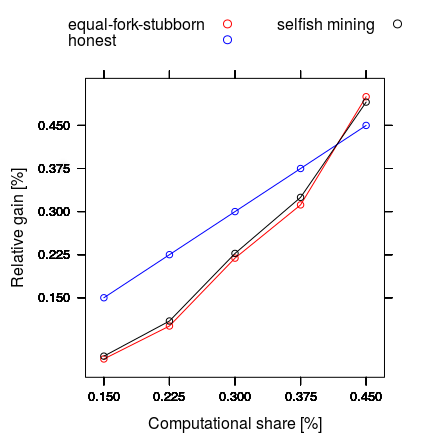
\includegraphics[width=12cm]{relative_block_share}
\centering
\caption{Relative revenue of the selfish miner}
\label{fig:relative_block_share}
\end{figure}

In figure \ref{fig:relative_block_share} the relative revenue, given a particular computation share and selfish mining strategy, is shown.
The graph shows that the two strategies selfish mining with \textit{lead stubborn, equal-fork stubborn} (\textit{L, F}) and selfish mining with all three modifications (\textit{L, F, T\textsubscript{1}}) are the worst performing strategies.
The relative share of accepted blocks of the two strategies stays clearly under the relative proportion which could be obtained by behaving honestly.
Also with an increase of the computational power the efficiency of the two selfish strategies is not amplified and the curve shows a linear progression.
The other six, better performing strategies are all exhibiting a similar behaviour.
The performance of these strategies is intensified with the augmentation of the computational share underlined by a concave curve.
Overall all selfish mining strategies are performing poorly and only with a computational share of about 40\% the six better performing strategies can retain a more significant share than the share obtained behaving honestly.
In table \ref{tab:relative_share_45} the relative  revenue share of the selfish miner with 45\% of computation power is shown.
The best performing strategies are equal-fork stubbornness (\textit{F}) and normal selfish mining (\textit{S}) followed by trail stubborn mining modified with equal-fork stubbornness \textit{F, T\textsubscript{1}} and the strategy trail stubborn (\textit{T\textsubscript{1}}).
These four strategies achieve almost similar results and are only 3\% apart.

\begin{table}
  \centering
  \begin{tabular}{cccc}
    \toprule
    strategy & share selfish & rank & difference to best\\
    \midrule
    F & 50\% & 1 & - \\
    S & 49.1\% & 2 & 0.9\% \\
    F, T\textsubscript{1} & 48.7\% & 3 & 1.3\% \\
    T\textsubscript{1} & 47\% & 4 & 3\% \\
    L & 45.4\% & 5 & 4.6\% \\
    L, T\textsubscript{1} & 45.3\% & 6 & 4.7\% \\
    H & 45\% & 7 & 5\% \\
    L, F, T\textsubscript{1} & 35.1\% & 8 & 14.9\% \\
    L, F & 33.8\% & 9 & 16.2\% \\
    \bottomrule
  \end{tabular}
  \caption{Relative share of selfish miner with 45\% of computational share}
  \label{tab:relative_share_45}
\end{table}

\begin{figure}[t]
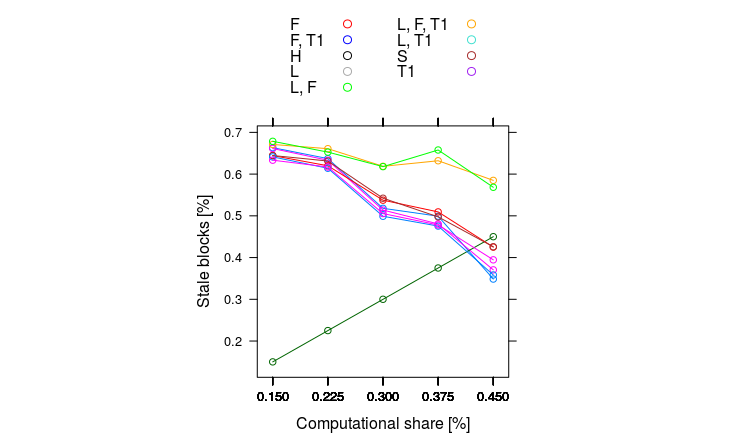
\includegraphics[width=12cm]{stale_blocks}
\centering
\caption{Share of stale blocks created by the selfish miner}
\label{fig:stale_blocks}
\end{figure}

Figure \ref{fig:stale_blocks} shows the share of stale blocks found by the selfish miner.
In the honest case, the share of created stale blocks increases linearly with the computational share.
Contrary to the line showing the honest behaviour proceed the lines depicting the different selfish mining strategies.
Especially if the computational share is low, over 60\% of the stale blocks of the network are created by the selfish miner.
With an increasing share of computational power, the share of stale blocks declines significantly, except the two strategies lead stubborn combined with equal-fork stubborn (\textit{L, F}) and selfish mining modified with all stubborn variations (\textit{L, F, T\textsubscript{1}}) which remain on the same level.
Additionally, the figure shows that only with a very high amount of computational share the selfish strategies are achieving better results than the normal, honest behaviour.

\begin{figure}[t]
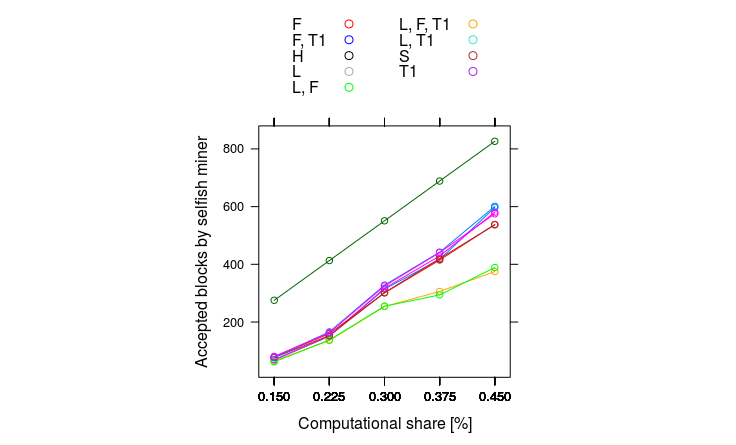
\includegraphics[width=12cm]{accepted_blocks_selfish}
\centering
\caption{Blocks created by the selfish miner and accepted in the longest chain}
\label{fig:accepted_blocks_selfish}
\end{figure}

The total amount of accepted blocks by the selfish miner, given a particular strategy and computational share, is shown in figure \ref{fig:accepted_blocks_selfish}.
The graph shows again the gap between the two bad performing strategies and the six other strategies which work slightly better.
Additionally, it can be seen that the absolute amount of accepted blocks during the execution of selfish mining is significantly lower than the number of blocks accepted when the nodes behave honestly.
Hence, in the short-run, all selfish mining strategies are yielding less mining rewards for the selfish miner than the normal, honest behaviour.

\begin{figure}[t]
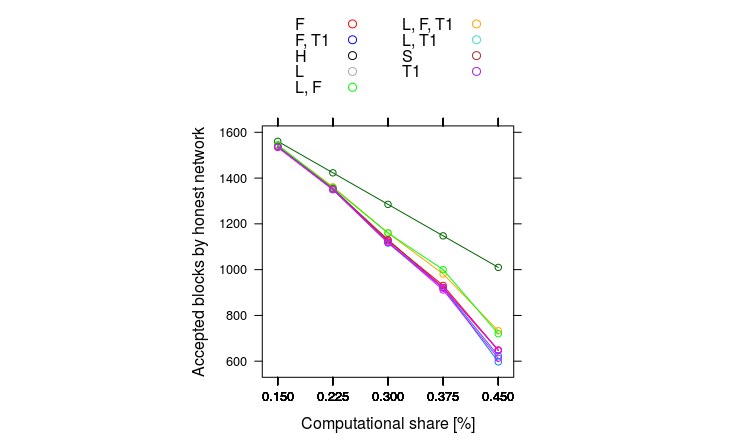
\includegraphics[width=12cm]{accepted_blocks_honest}
\centering
\caption{Blocks created by the honest network and accepted in the longest chain}
\label{fig:accepted_blocks_honest}
\end{figure}

The honest network also creates less accepted blocks during a selfish mining attack as shown in figure \ref{fig:accepted_blocks_honest}.
Since the selfish mining strategies are functioning better with an increasing computational share of the selfish miner, the gap between the case where all nodes behave honestly and the case where one node conducts selfish mining even increases.
The performance differences between the selfish mining strategies can also be seen in this figure.

\begin{figure}[t]
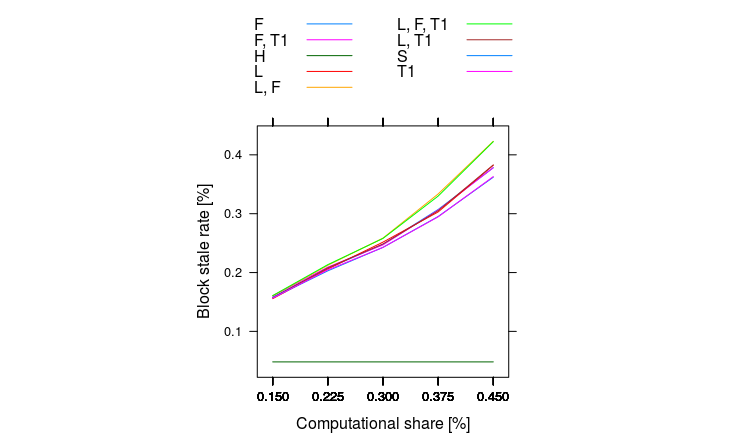
\includegraphics[width=12cm]{stale_rate}
\centering
\caption{Stale block rate}
\label{fig:stale_rate}
\end{figure}

Lastly, in figure \ref{fig:stale_rate} the relative amount of stale blocks in the network during the simulations is shown.
If all nodes behave honestly, the stale block rate is 4.821\% as measured during the evaluation of the simulation software.
In the case that a node conducts a selfish mining strategy the stale block rate is significantly higher and increases further if the computational power of the selfish miner is augmented.
Furthermore, the gap between the two worst performing selfish strategies and the other strategies can be observed.
If a node conducts lead stubbornness combined with equal-fork stubbornness (\textit{L, F}) or selfish mining with all three modifications (\textit{L, F, T\textsubscript{1}}), there are even more stale blocks in the network.

Similar as during the evaluation of the deterministic behaviour of the simulation software in chapter 45, also during the execution of the selfish mining scenarios the utilisation of the CPU and the memory of the host machine stayed under 10\% as shown in figure \ref{fig:selfish_simulations_cpu} and figure \ref{fig:selfish_simulations_memory}.
Thus, the specifications of the host machine did not restrict the simulations in any way.

\begin{figure}[t]
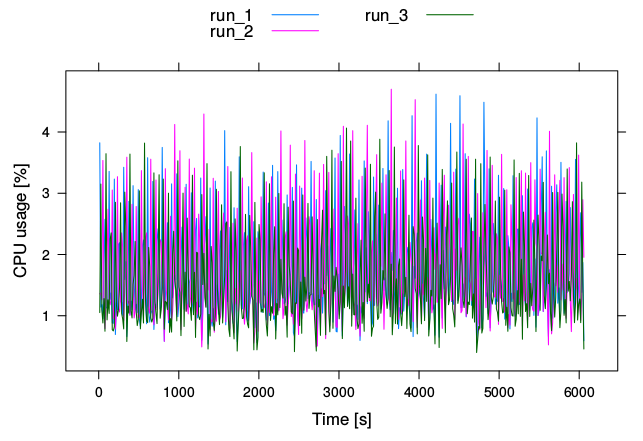
\includegraphics[width=8cm]{selfish_simulations_cpu}
\centering
\caption{CPU usage during the triple execution of a simulation scenario}
\label{fig:selfish_simulations_cpu}
\end{figure}

\begin{figure}[t]
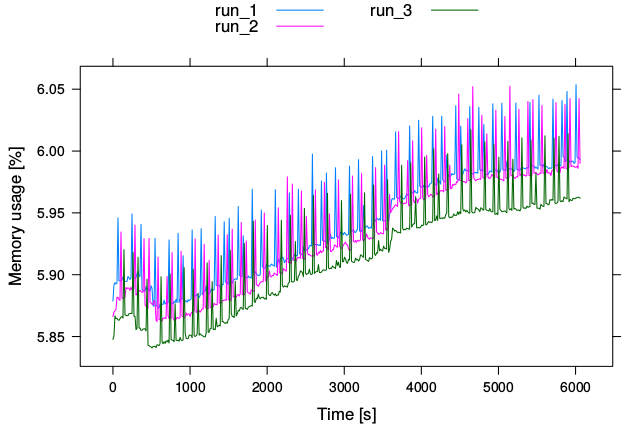
\includegraphics[width=8cm]{selfish_simulations_memory}
\centering
\caption{Memory usage during the triple execution of a simulation scenario}
\label{fig:selfish_simulations_memory}
\end{figure}
